% ================================================================
% EMPIRICAL APPLICATION — Dominick's Analgesics
% Auto-generated by run_dominicks_experiments.py
% n\_runs = 5  (mean $\pm$ std across independent re-estimations)
% Packages: booktabs, threeparttable, graphicx, siunitx
% ================================================================

\begin{table}[htbp]
  \centering
  \caption{Descriptive Statistics: Dominick's Analgesics Scanner Panel}
  \label{tab:dom_desc}
  \begin{threeparttable}
    \begin{tabular}{lS[table-format=2.3]S[table-format=1.3]S[table-format=1.4]S[table-format=1.4]}
      \toprule
      \textbf{Good} & {\textbf{Mean Price}} & {\textbf{Std Price}} & {\textbf{Mean Share}} & {\textbf{Std Share}} \\
      & {(\$/100 tablets)} & & & \\
      \midrule
      Aspirin & 7.311 & 1.557 & 0.2107 & 0.0519 \\
      Acetaminophen & 10.554 & 1.427 & 0.5026 & 0.0785 \\
      Ibuprofen & 10.506 & 1.428 & 0.2867 & 0.0819 \\
      \midrule
      \multicolumn{5}{l}{\textit{Train: 28,644 obs\quad Test: 4,287 obs\quad Stores: 93\quad Weeks: 1--399}} \\
      \bottomrule
    \end{tabular}
    \begin{tablenotes}\small
      \item Unit prices standardised to per-100-tablet equivalent.
    \end{tablenotes}
  \end{threeparttable}
\end{table}

\begin{table}[htbp]
  \centering
  \caption{Out-of-Sample Predictive Accuracy --- Dominick's Analgesics (5 independent re-estimations; mean $\pm$ std)}
  \label{tab:dom_acc}
  \begin{threeparttable}
    \begin{tabular}{lcc}
      \toprule
      \textbf{Model} & \textbf{RMSE} & \textbf{MAE} \\
      \midrule
      LA-AIDS & $0.07069 \pm 0.00000$ & $0.05593 \pm 0.00000$ \\
      BLP (IV) & $0.07766 \pm 0.00000$ & $0.05991 \pm 0.00000$ \\
      QUAIDS & $0.06956 \pm 0.00000$ & $0.05519 \pm 0.00000$ \\
      Series Est. & $0.06514 \pm 0.00000$ & $0.05077 \pm 0.00000$ \\
      Neural Demand (window) & $0.08045 \pm 0.00107$ & $0.06348 \pm 0.00097$ \\
      LDS (Shared) & $0.09200 \pm 0.00000$ & $0.07360 \pm 0.00000$ \\
      LDS (GoodSpec) & $0.09197 \pm 0.00000$ & $0.07356 \pm 0.00000$ \\
      LDS (Orth) & $0.08679 \pm 0.00000$ & $0.07061 \pm 0.00000$ \\
      Neural Demand (static) & $0.06450 \pm 0.00044$ & $0.04990 \pm 0.00026$ \\
      Neural Demand (habit) & $0.04787 \pm 0.00010$ & $0.03592 \pm 0.00010$ \\
      Var. Mixture & $0.09407 \pm 0.01496$ & $0.07852 \pm 0.01329$ \\
      Neural Demand (FE) & $0.05861 \pm 0.00062$ & $0.04475 \pm 0.00056$ \\
      Neural Demand (habit, FE) & $0.04801 \pm 0.00010$ & $0.03609 \pm 0.00014$ \\
      Neural Demand (CF) & $0.06715 \pm 0.00048$ & $0.05133 \pm 0.00032$ \\
      \textbf{Neural Demand (habit, CF)} & \textbf{$0.04785 \pm 0.00032$} & $0.03602 \pm 0.00028$ \\
      Neural Demand (habit, FE, CF) & $0.04788 \pm 0.00021$ & $0.03598 \pm 0.00015$ \\
      \bottomrule
    \end{tabular}
    \begin{tablenotes}\small
      \item RMSE and MAE on held-out test observations, mean $\pm$ std over 5 run(s).
    \end{tablenotes}
  \end{threeparttable}
\end{table}

\begin{table}[htbp]
  \centering
  \caption{Own-Price Quantity Elasticities --- Dominick's Analgesics (5 run(s); mean $\pm$ std)}
  \label{tab:dom_elast}
  \begin{threeparttable}
    \begin{tabular}{lccc}
      \toprule
      \textbf{Model} & {$\hat{\varepsilon}_{00}$ (Aspirin)} & {$\hat{\varepsilon}_{11}$ (Acetaminophen)} & {$\hat{\varepsilon}_{22}$ (Ibuprofen)} \\
      \midrule
      LA-AIDS & $-0.849 \pm 0.000$ & $-1.420 \pm 0.000$ & $-1.140 \pm 0.000$ \\
      BLP (IV) & $-0.998 \pm 0.000$ & $-1.769 \pm 0.000$ & $-0.587 \pm 0.000$ \\
      QUAIDS & $-0.882 \pm 0.000$ & $-1.423 \pm 0.000$ & $-1.129 \pm 0.000$ \\
      Series Est. & $-0.708 \pm 0.000$ & $-1.629 \pm 0.000$ & $-1.224 \pm 0.000$ \\
      Neural Demand (window) & $-0.982 \pm 0.007$ & $-1.186 \pm 0.010$ & $-1.437 \pm 0.017$ \\
      LDS (Shared) & $-0.163 \pm 0.000$ & $-0.214 \pm 0.000$ & $-0.189 \pm 0.000$ \\
      LDS (GoodSpec) & $-0.164 \pm 0.000$ & $-0.205 \pm 0.000$ & $-0.181 \pm 0.000$ \\
      LDS (Orth) & $-1.157 \pm 0.000$ & $-1.119 \pm 0.000$ & $-1.168 \pm 0.000$ \\
      Neural Demand (static) & $-0.711 \pm 0.030$ & $-1.562 \pm 0.021$ & $-1.273 \pm 0.022$ \\
      Neural Demand (habit) & $-0.930 \pm 0.008$ & $-1.233 \pm 0.020$ & $-1.175 \pm 0.015$ \\
      Var. Mixture & $-1.508 \pm 0.146$ & $-1.363 \pm 0.105$ & $-1.547 \pm 0.197$ \\
      Neural Demand (FE) & $-0.936 \pm 0.035$ & $-1.448 \pm 0.028$ & $-0.965 \pm 0.034$ \\
      Neural Demand (habit, FE) & $-0.921 \pm 0.015$ & $-1.232 \pm 0.014$ & $-1.134 \pm 0.009$ \\
      Neural Demand (CF) & $-0.840 \pm 0.033$ & $-1.515 \pm 0.021$ & $-0.949 \pm 0.019$ \\
      Neural Demand (habit, CF) & $-0.972 \pm 0.015$ & $-1.305 \pm 0.015$ & $-1.246 \pm 0.023$ \\
      Neural Demand (habit, FE, CF) & $-0.959 \pm 0.017$ & $-1.275 \pm 0.011$ & $-1.215 \pm 0.023$ \\
      \bottomrule
    \end{tabular}
    \begin{tablenotes}\small
      \item Numerical own-price quantity elasticities at mean test prices.
    \end{tablenotes}
  \end{threeparttable}
\end{table}

\begin{table}[htbp]
  \centering
  \caption{Consumer Surplus Loss from 10\% Ibuprofen Price Increase --- Dominick\'s Analgesics (5 run(s); mean $\pm$ std)}
  \label{tab:dom_welfare}
  \begin{threeparttable}
    \begin{tabular}{lcr}
      \toprule
      \textbf{Model} & \textbf{CV Loss (\$)} & \textbf{vs Neural Demand (static)} \\
      \midrule
      LA-AIDS & $-0.2322 \pm 0.0000$ & +1.4\% \\
      BLP (IV) & $-0.2212 \pm 0.0000$ & +6.1\% \\
      QUAIDS & $-0.2339 \pm 0.0000$ & +0.7\% \\
      Series Est. & $-0.2333 \pm 0.0000$ & +1.0\% \\
      Neural Demand (window) & $-0.2386 \pm 0.0015$ & -1.3\% \\
      LDS (Shared) & $-0.2823 \pm 0.0000$ & -19.8\% \\
      LDS (GoodSpec) & $-0.2818 \pm 0.0000$ & -19.6\% \\
      LDS (Orth) & $-0.2409 \pm 0.0000$ & -2.3\% \\
      Neural Demand (static) & $-0.2355 \pm 0.0030$ &  \\
      Neural Demand (habit) & $-0.2130 \pm 0.0014$ & +9.6\% \\
      Var. Mixture & $-0.2988 \pm 0.0347$ & -26.8\% \\
      Neural Demand (FE) & $-0.2392 \pm 0.0024$ & -1.5\% \\
      Neural Demand (habit, FE) & $-0.2217 \pm 0.0013$ & +5.9\% \\
      Neural Demand (CF) & $-0.2253 \pm 0.0037$ & +4.3\% \\
      Neural Demand (habit, CF) & $-0.2143 \pm 0.0024$ & +9.0\% \\
      Neural Demand (habit, FE, CF) & $-0.2206 \pm 0.0027$ & +6.3\% \\
      \bottomrule
    \end{tabular}
    \begin{tablenotes}\small
      \item Compensating variation via 100-step Riemann sum, $p_{\mathrm{Ibu}}\to(1+0.1)\,p_{\mathrm{Ibu}}$.
    \end{tablenotes}
  \end{threeparttable}
\end{table}

\begin{table}[htbp]
  \centering
  \caption{MDP State Augmentation: Brand Loyalty in Analgesic Demand (5 run(s); mean $\pm$ std)}
  \label{tab:dom_mdp}
  \begin{threeparttable}
    \begin{tabular}{lcccc}
      \toprule
      \textbf{Model} & \textbf{RMSE} & \textbf{KL Div.} & \textbf{Reduction} \\
      \midrule
      LA-AIDS & $0.07069 \pm 0.00000$ & $0.02311 \pm 0.00000$ & baseline \\
      Neural Demand (static) & $0.06450 \pm 0.00044$ & $0.01969 \pm 0.00029$ & 8.8% \\
      Neural Demand (habit) & $0.04787 \pm 0.00010$ & $0.01060 \pm 0.00006$ & 32.3% \\
      Neural Demand (CF) & $0.06715 \pm 0.00048$ & $0.02080 \pm 0.00026$ & 5.0% \\
      Neural Demand (habit, CF) & $0.04785 \pm 0.00032$ & $0.01063 \pm 0.00017$ & 32.3% \\
      \bottomrule
    \end{tabular}
    \begin{tablenotes}\small
      \item Habit-decay $\hat{\delta}$ (habit model) = 0.868$\pm$0.002; FE variant: 0.860$\pm$0.005.
      RMSE and KL: mean $\pm$ std over 5 independent re-estimation(s).
    \end{tablenotes}
  \end{threeparttable}
\end{table}

\begin{table}[htbp]
  \centering
  \caption{Variational Mixture IRL: Consumer Segments --- Dominick\'s Analgesics ($K=6$; last of 5 run(s))}
  \label{tab:dom_mix}
  \begin{threeparttable}
    \begin{tabular}{cS[table-format=1.3]S[table-format=1.3]S[table-format=1.3]S[table-format=1.3]S[table-format=1.3]l}
      \toprule
      $k$ & {$\hat{\pi}_k$} & {$\hat{\alpha}_{\text{Asp}}$} & {$\hat{\alpha}_{\text{Acet}}$} & {$\hat{\alpha}_{\text{Ibu}}$} & {$\hat{\rho}$} & Segment \\
      \midrule
      1 & 0.028 & 0.262 & 0.349 & 0.389 & 0.300 & Balanced \\
      2 & 0.874 & 0.292 & 0.388 & 0.320 & 0.362 & \textbf{Dominant / mixed} \\
      3 & 0.028 & 0.345 & 0.294 & 0.361 & 0.420 & Balanced \\
      4 & 0.017 & 0.334 & 0.305 & 0.361 & 0.480 & Balanced \\
      5 & 0.031 & 0.335 & 0.301 & 0.364 & 0.540 & Balanced \\
      6 & 0.022 & 0.384 & 0.377 & 0.239 & 0.600 & Price-sensitive switchers \\
      \bottomrule
    \end{tabular}
    \begin{tablenotes}\small
      \item Gaussian mixture in $(\bm{\alpha},\rho)$ CES parameter space.
    \end{tablenotes}
  \end{threeparttable}
\end{table}

\begin{figure}[htbp]
  \centering
  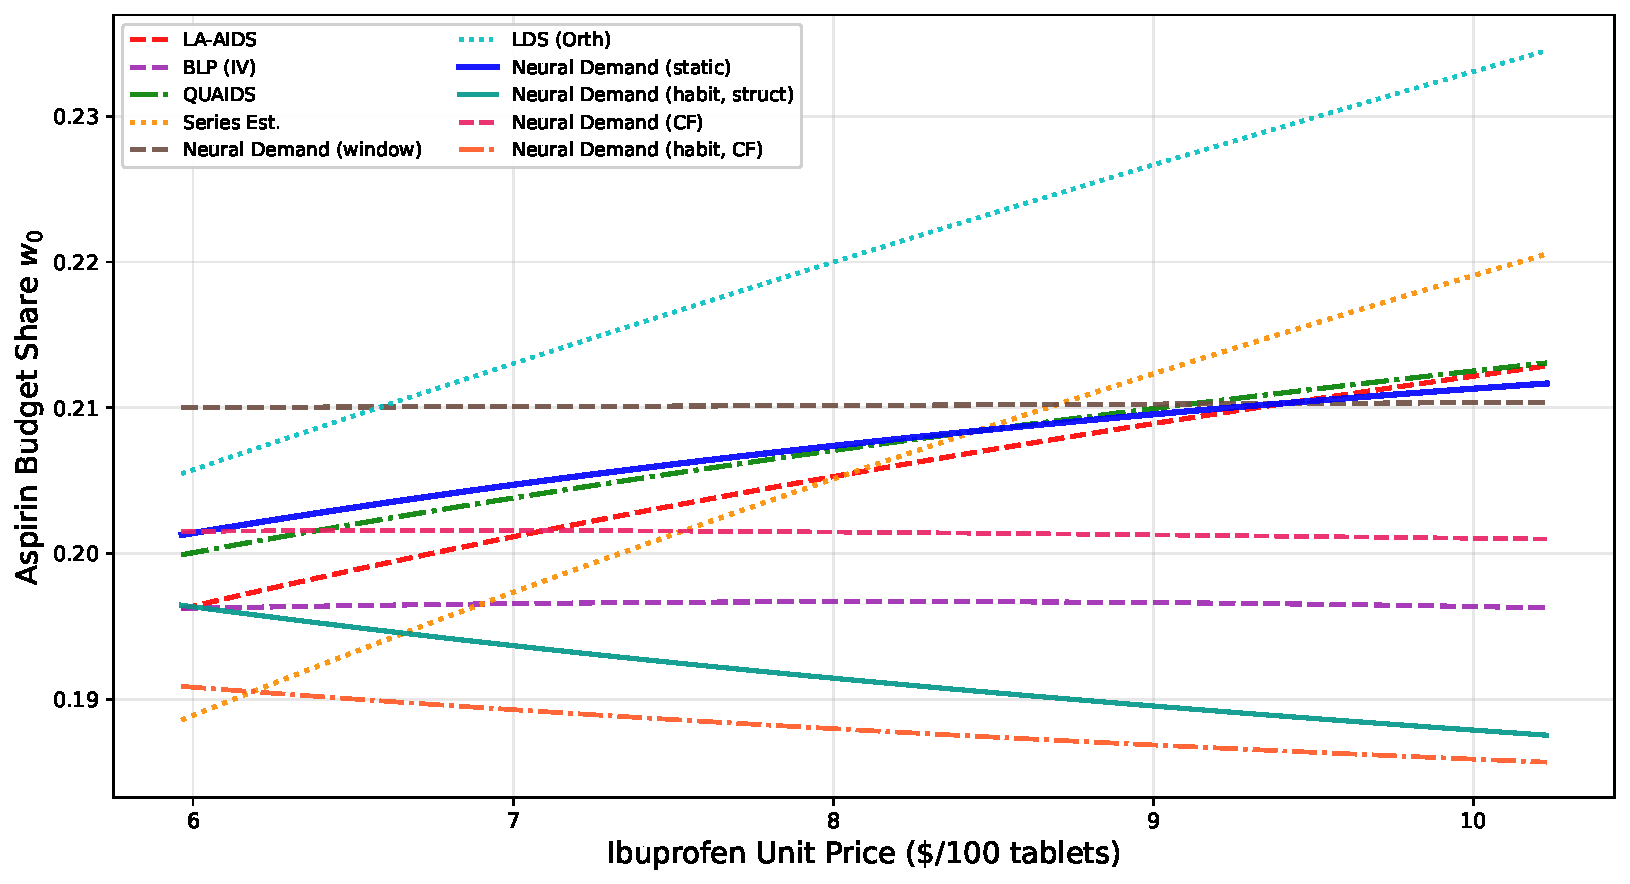
\includegraphics[width=\textwidth]{results/neural_demand/dominicks/figures/fig_demand_curves.pdf}
  \caption{Aspirin Budget Share as a Function of Ibuprofen Unit Price --- Dominick's Analgesics. Shaded bands indicate $\pm 1$ standard deviation across 5 independent re-estimations.}
  \label{fig:dom_demand}
\end{figure}

\begin{figure}[htbp]
  \centering
  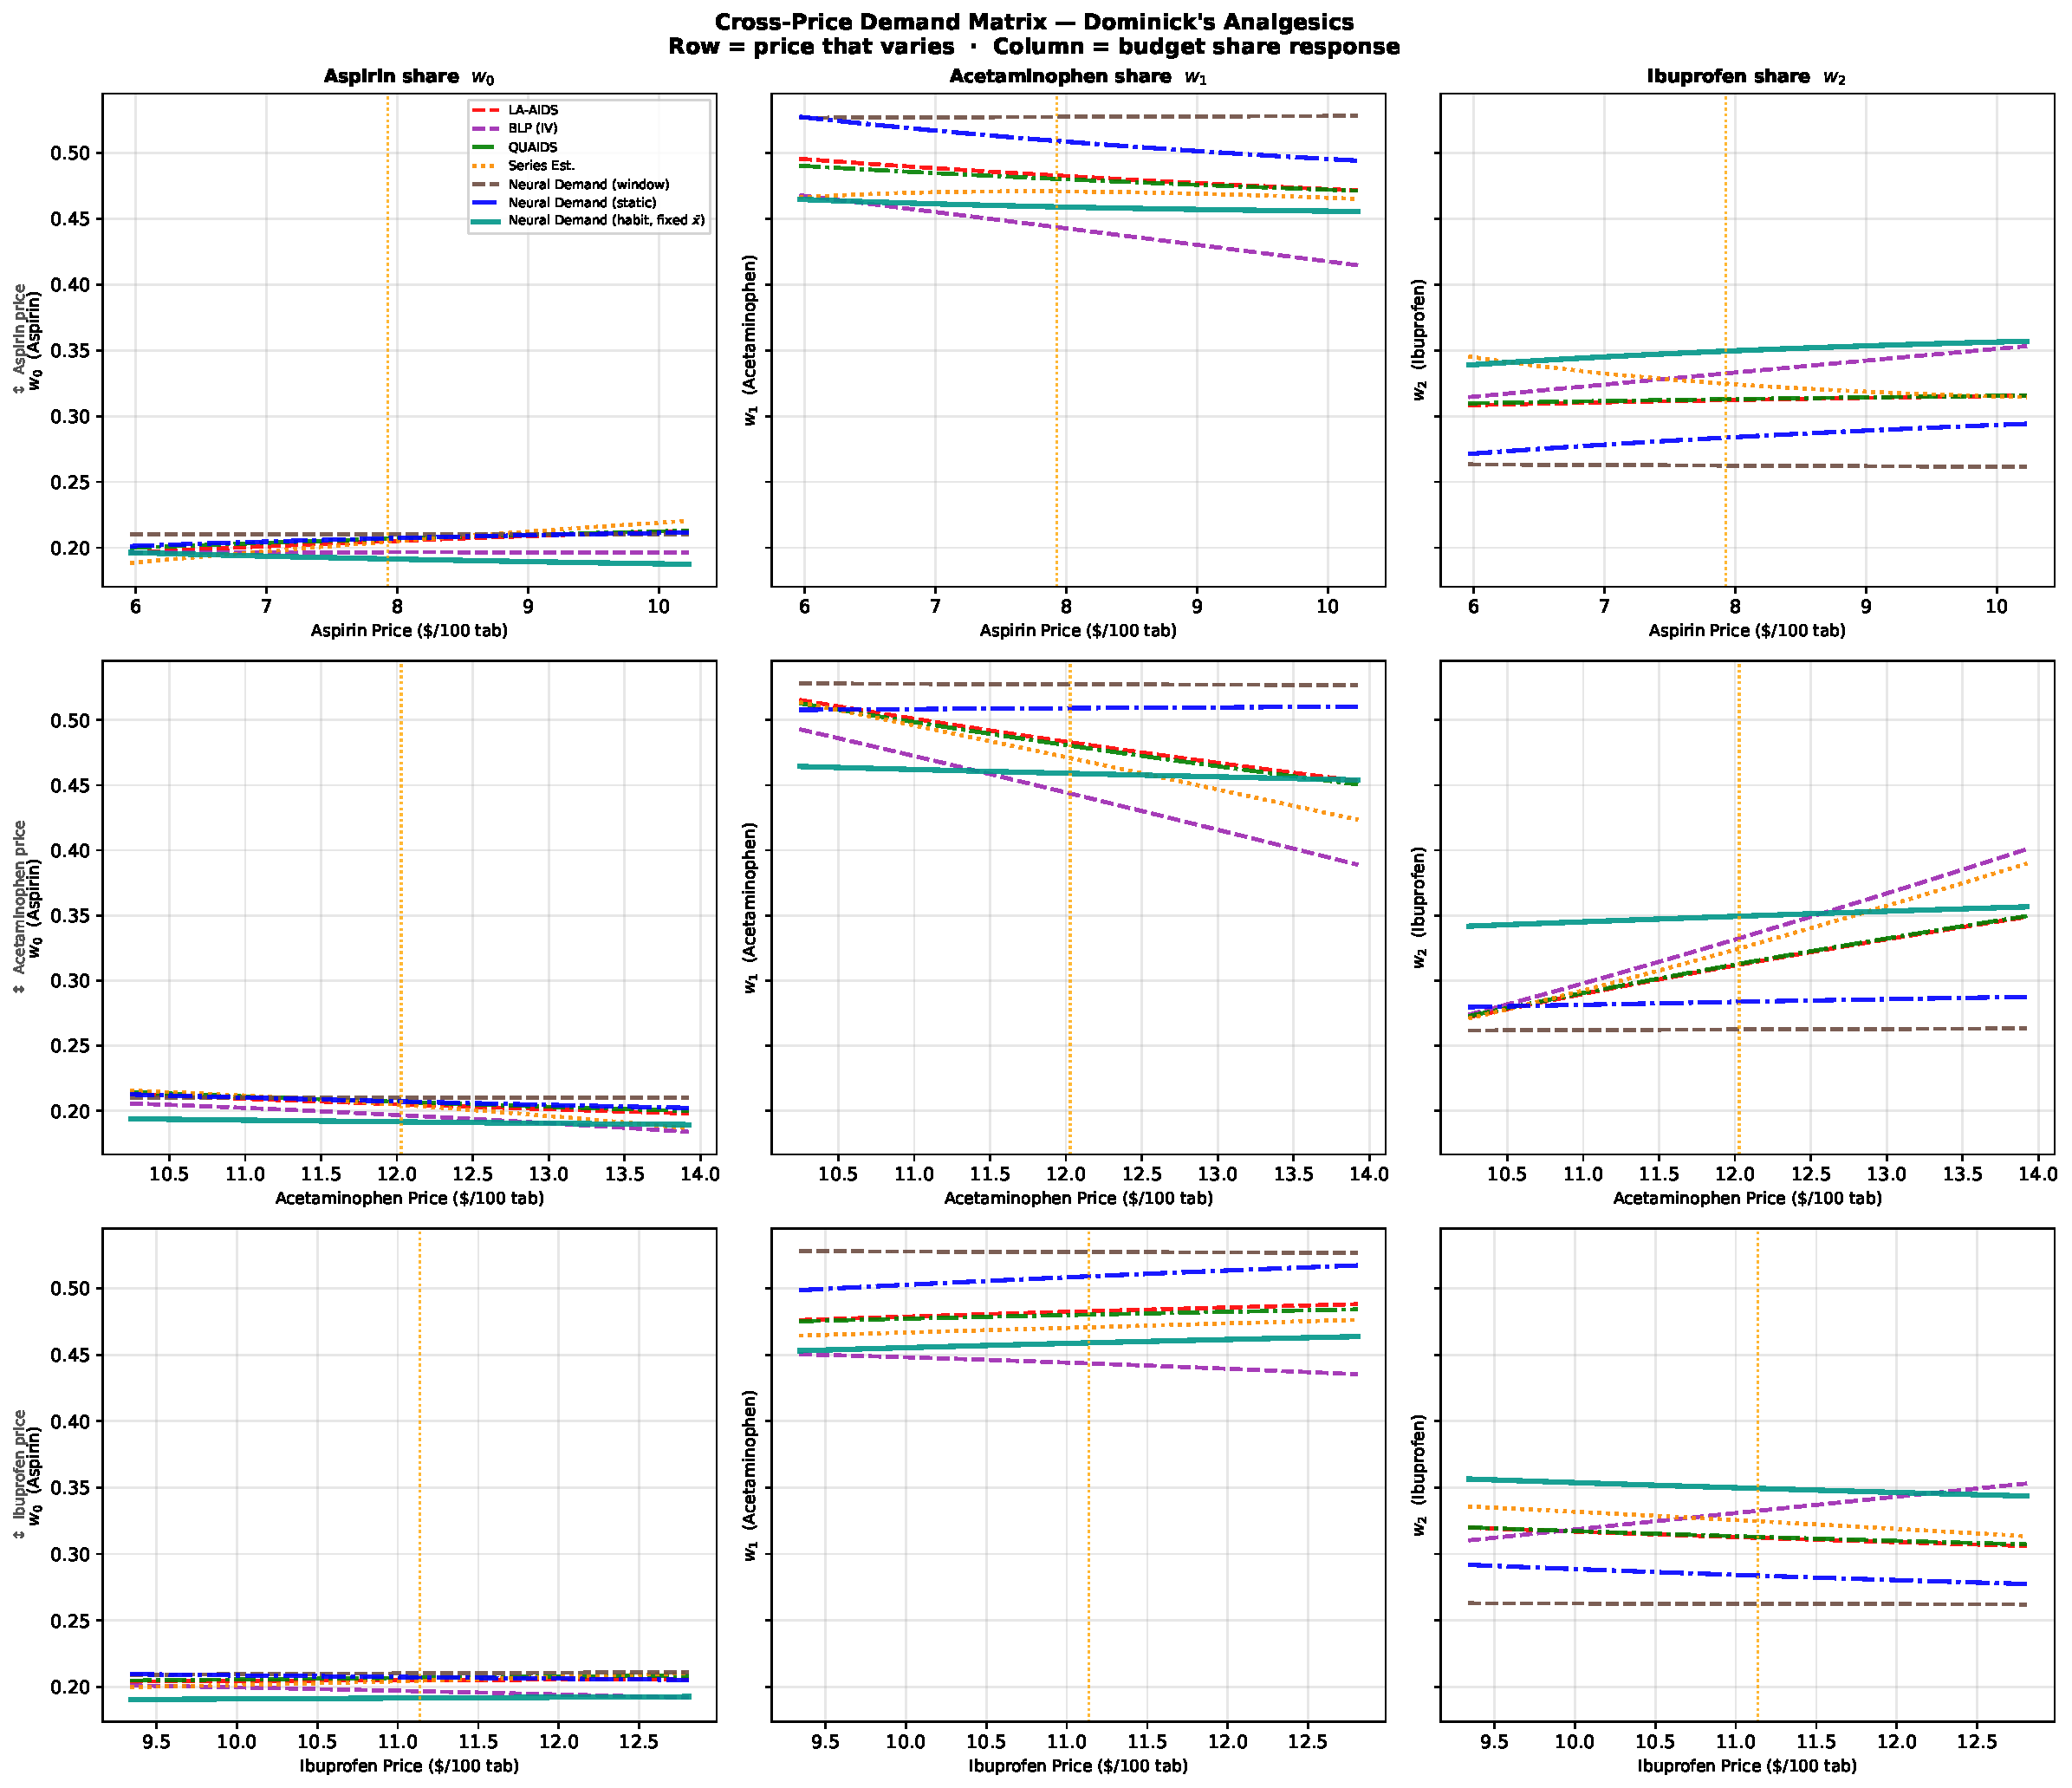
\includegraphics[width=\textwidth]{results/neural_demand/dominicks/figures/fig_mdp_advantage.pdf}
  \caption{Cross-Price Demand Matrix — Dominick's Analgesics. Shaded bands indicate $\pm 1$ standard deviation across 5 independent re-estimations.}
  \label{fig:dom_mdp}
\end{figure}

\begin{figure}[htbp]
  \centering
  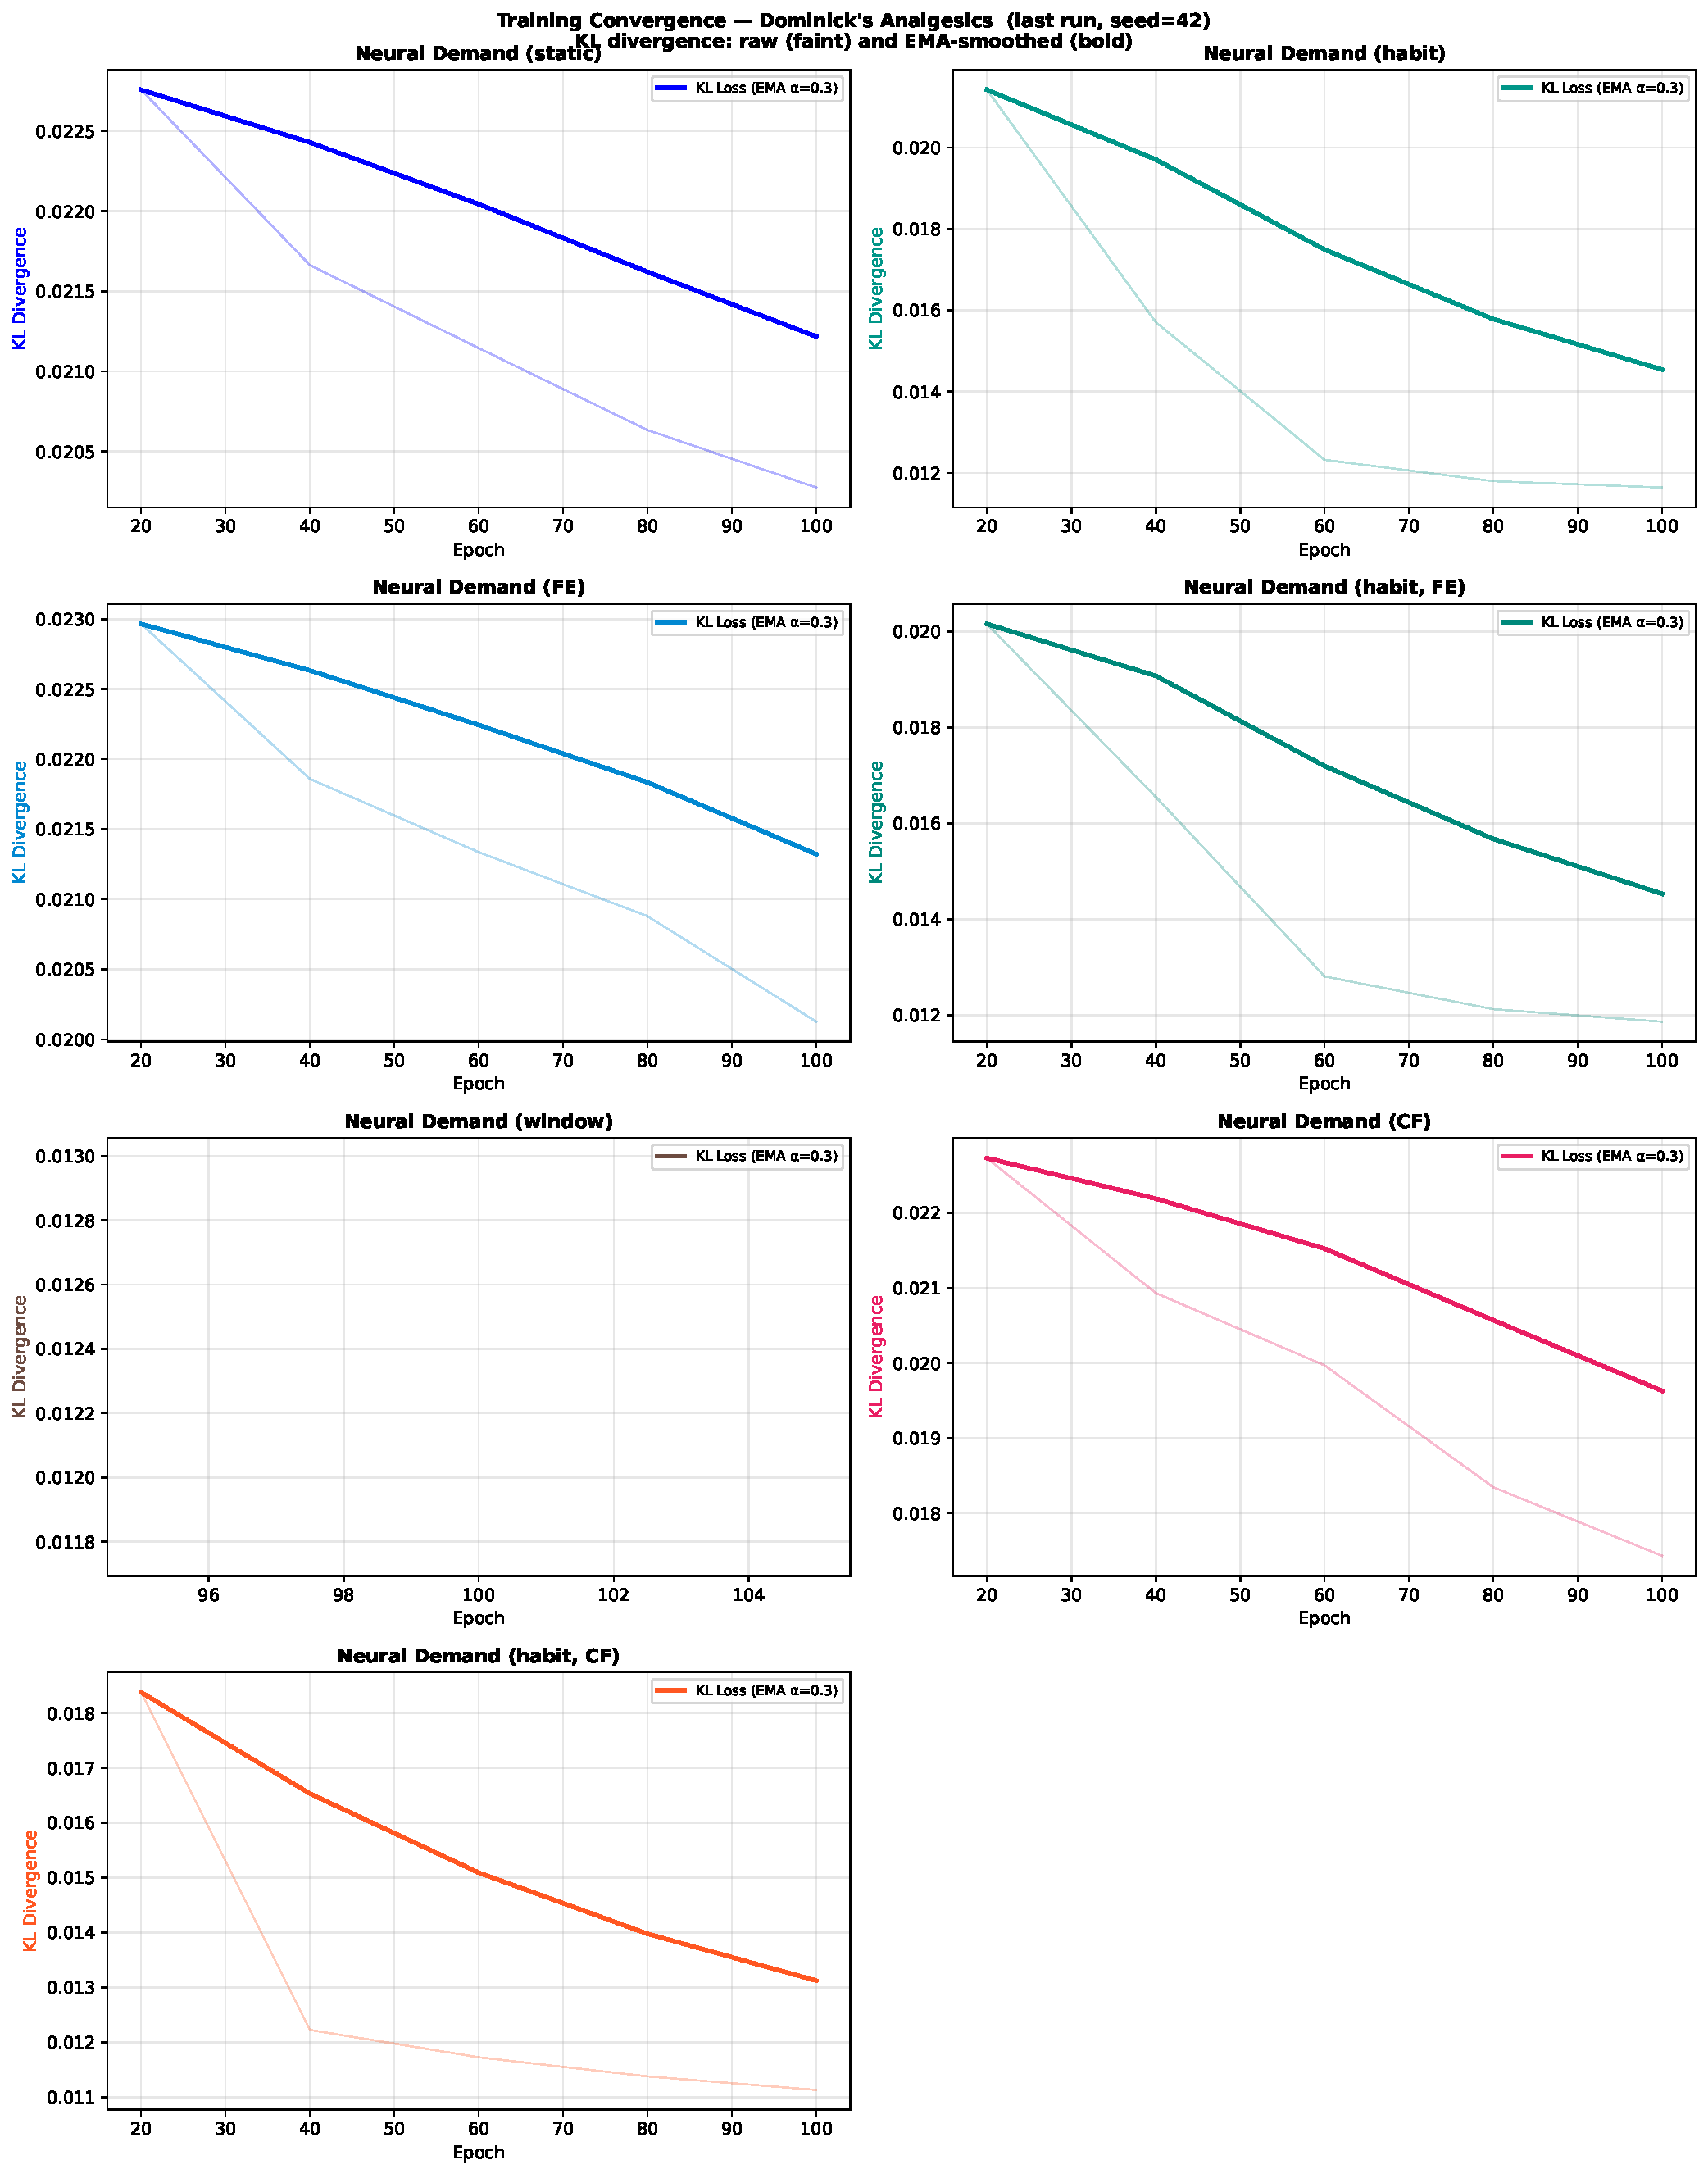
\includegraphics[width=\textwidth]{results/neural_demand/dominicks/figures/fig_convergence.pdf}
  \caption{Training Convergence — Dominick's Analgesics (last run).}
  \label{fig:dom_conv}
\end{figure}

\begin{figure}[htbp]
  \centering
  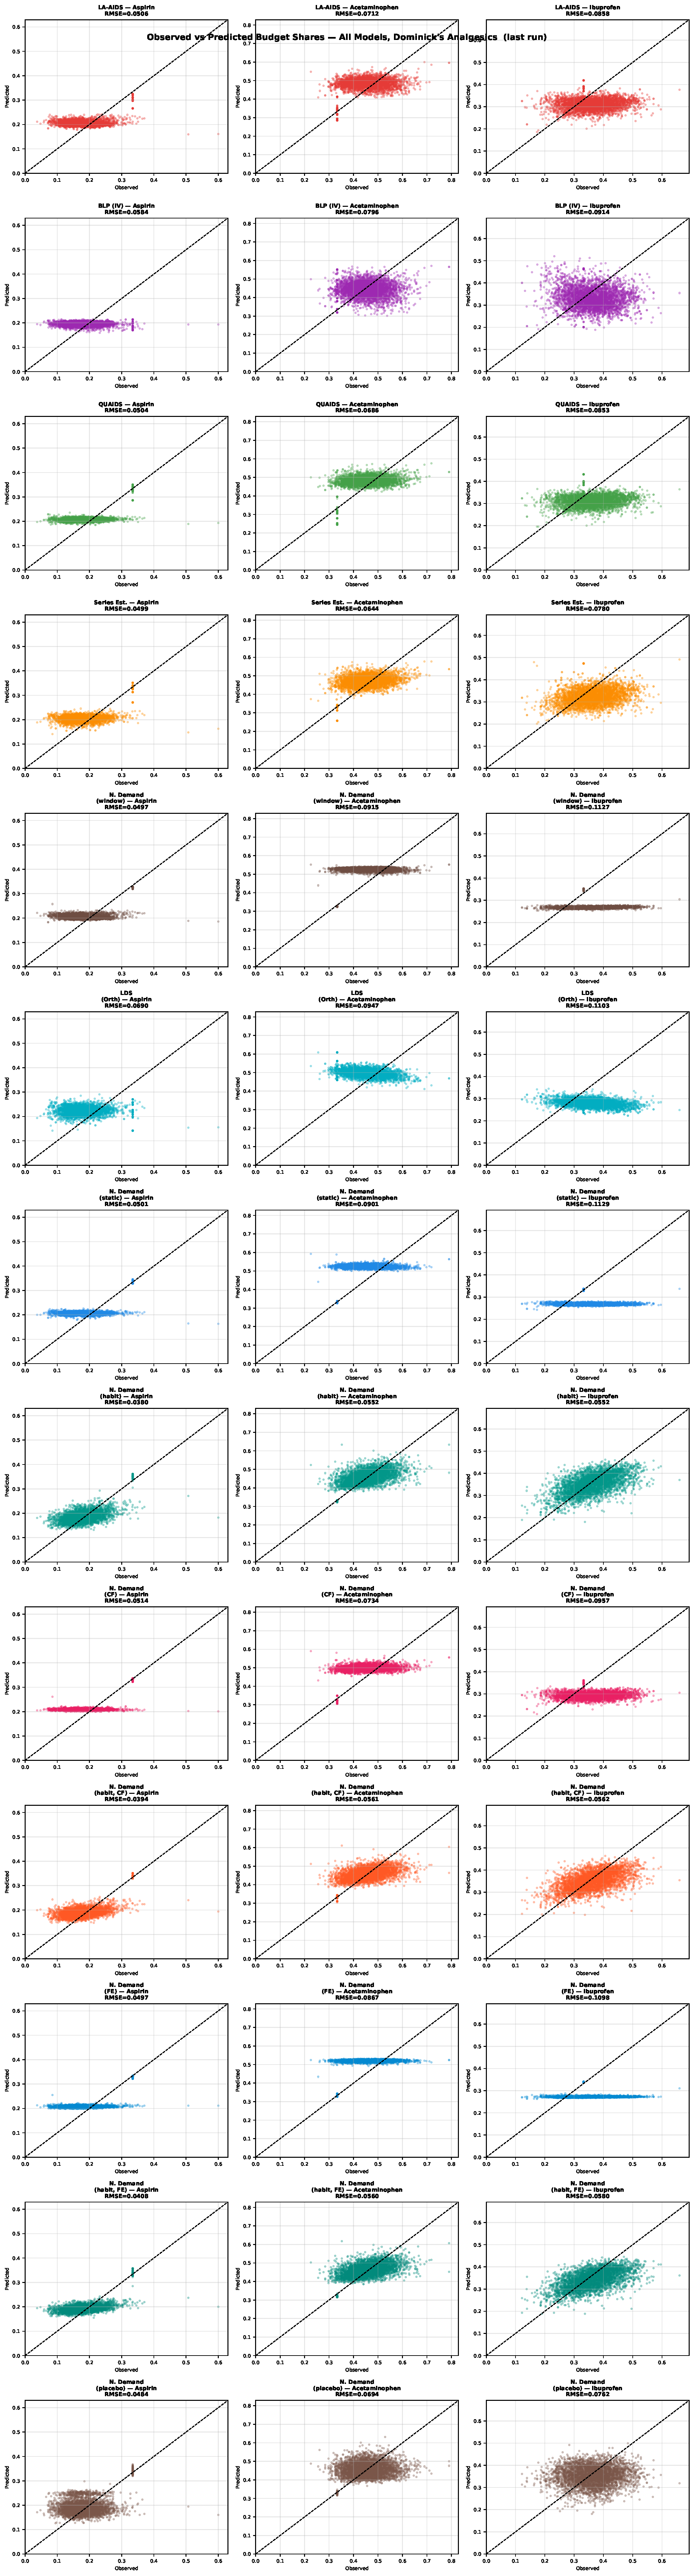
\includegraphics[width=\textwidth]{results/neural_demand/dominicks/figures/fig_scatter.pdf}
  \caption{Observed vs. Predicted Budget Shares — Dominick's Analgesics (last run).}
  \label{fig:dom_scatter}
\end{figure}

\begin{figure}[htbp]
  \centering
  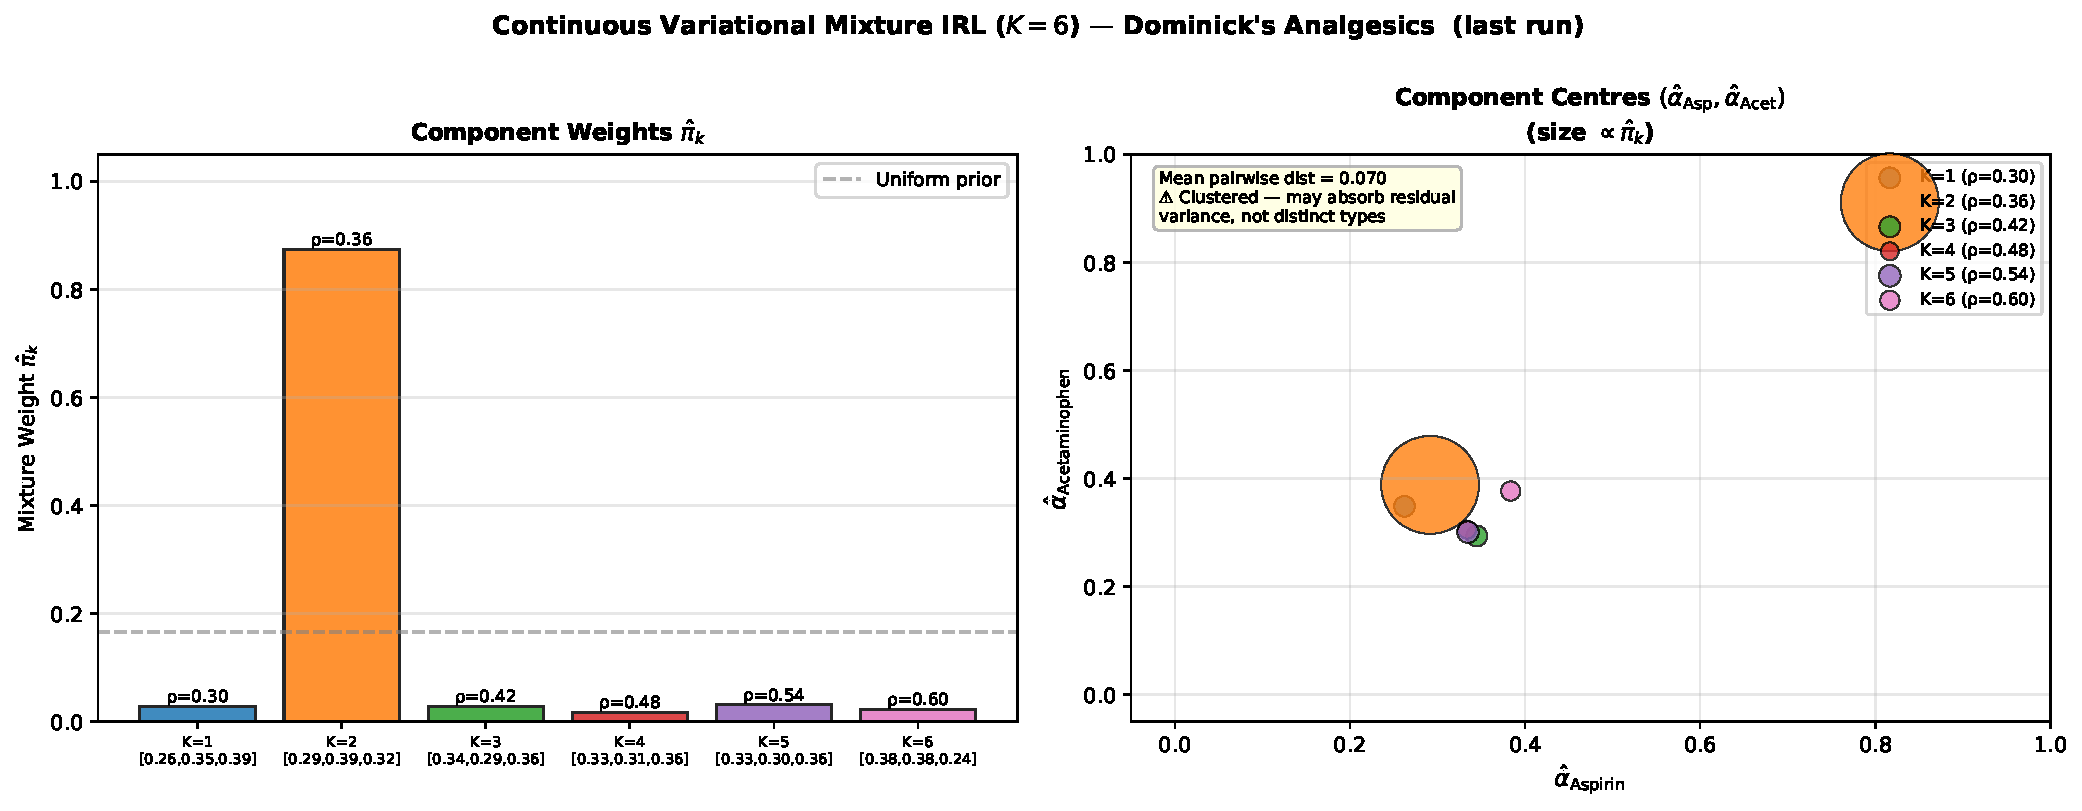
\includegraphics[width=\textwidth]{results/neural_demand/dominicks/figures/fig_mixture.pdf}
  \caption{Continuous Variational Mixture IRL ($K=6$) — Dominick's Analgesics (last run).}
  \label{fig:dom_mix}
\end{figure}

\begin{figure}[htbp]
  \centering
  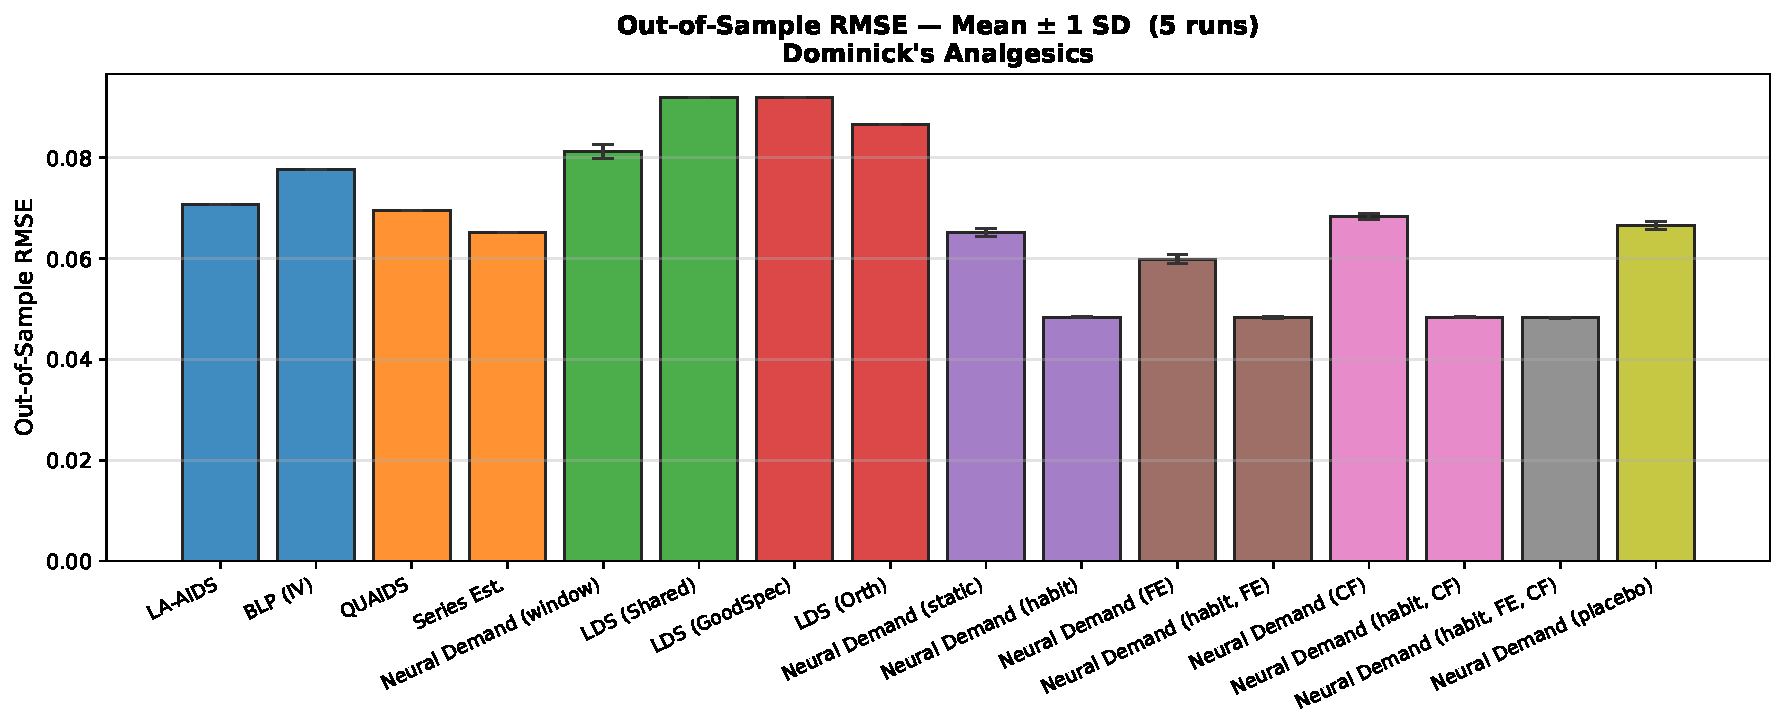
\includegraphics[width=\textwidth]{results/neural_demand/dominicks/figures/fig_rmse_bars.pdf}
  \caption{Out-of-Sample RMSE across all models — mean $\pm 1$ SD over 5 runs.}
  \label{fig:dom_rmse_bars}
\end{figure}

\begin{figure}[htbp]
  \centering
  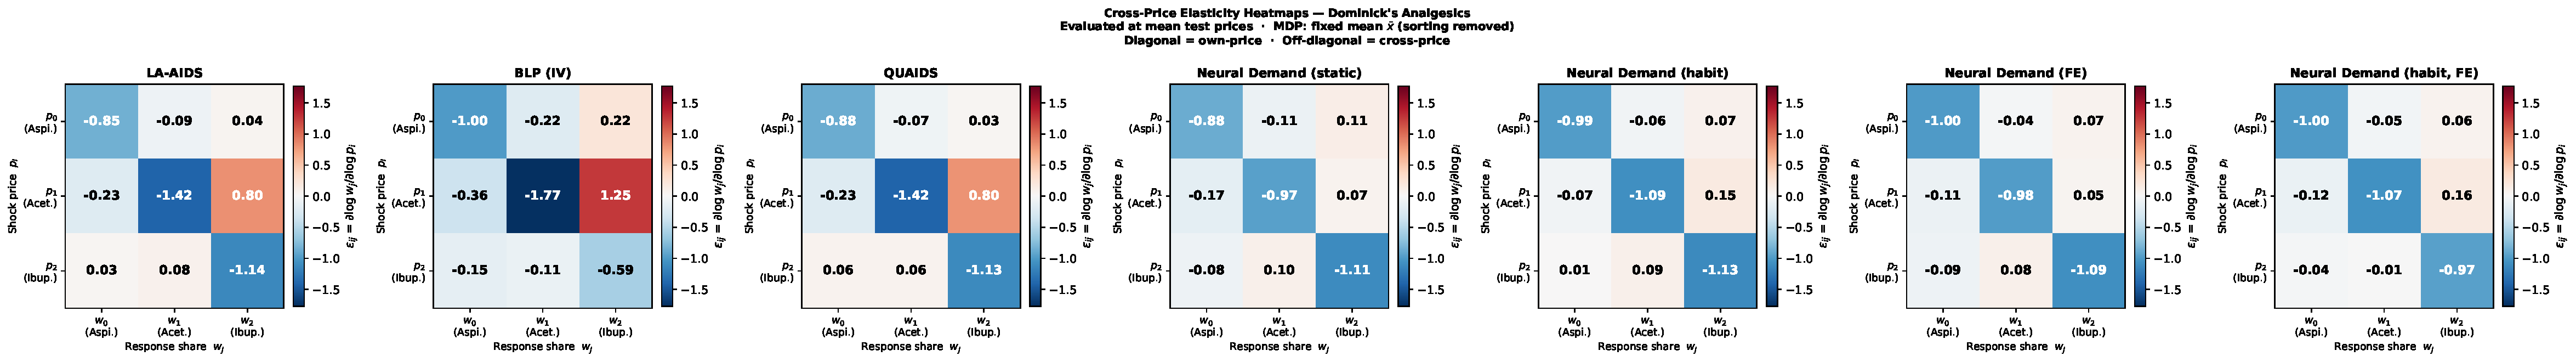
\includegraphics[width=\textwidth]{results/neural_demand/dominicks/figures/fig_cross_elast_heatmap.pdf}
  \caption{Cross-Price Elasticity Heatmaps.}
  \label{fig:dom_cross_elast}
\end{figure}

\begin{figure}[htbp]
  \centering
  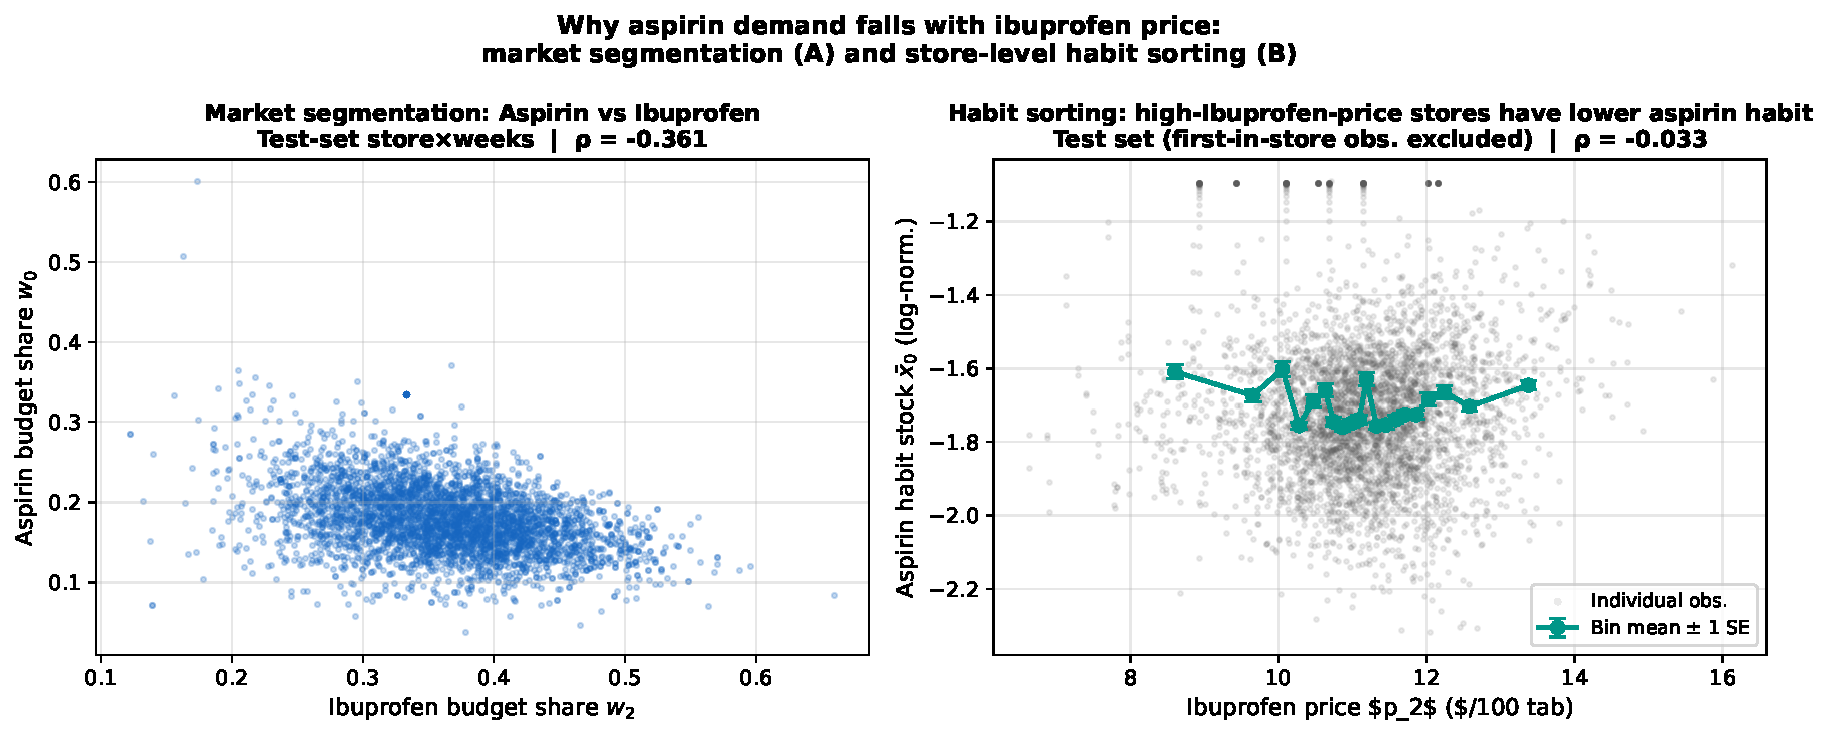
\includegraphics[width=\textwidth]{results/neural_demand/dominicks/figures/fig_segmentation_sorting.pdf}
  \caption{Market segmentation and habit-sorting diagnostics.}
  \label{fig:dom_sorting}
\end{figure}

\begin{figure}[htbp]
  \centering
  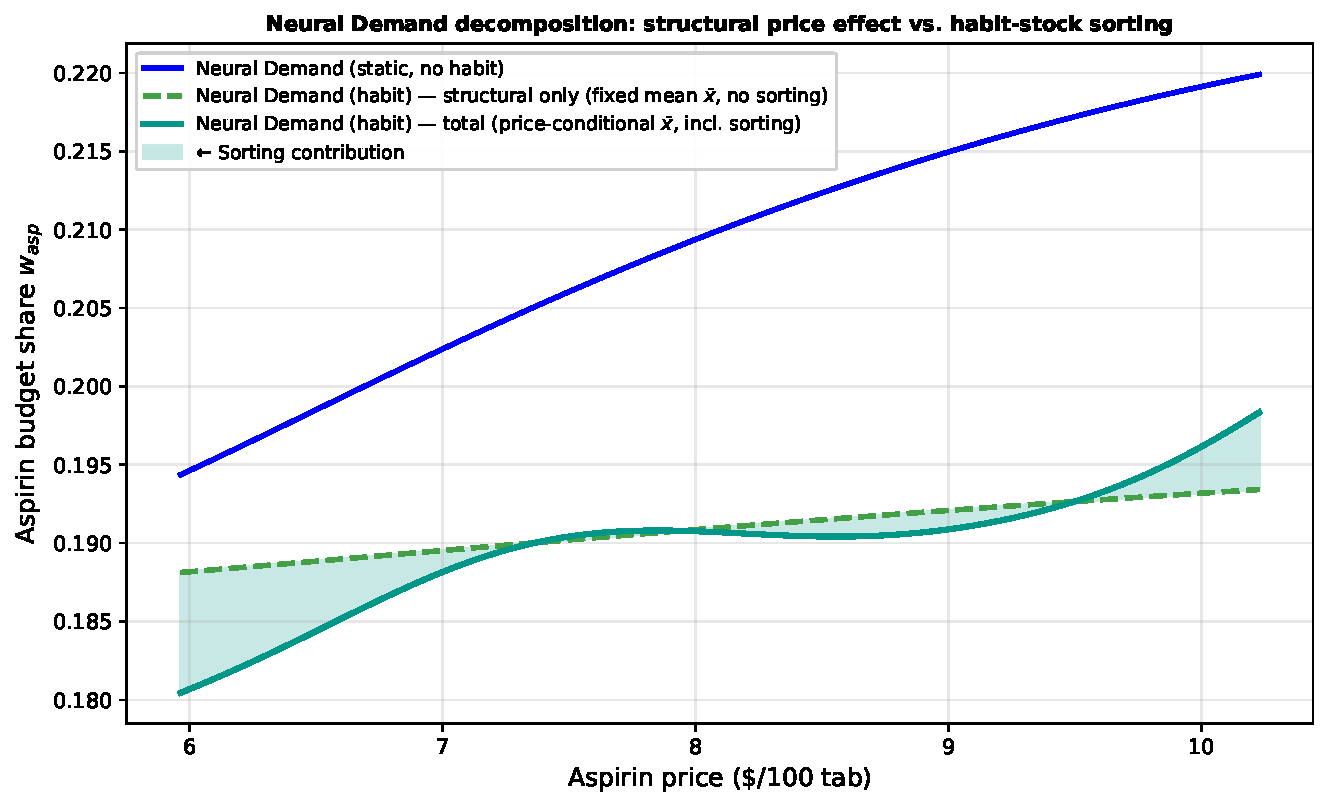
\includegraphics[width=\textwidth]{results/neural_demand/dominicks/figures/fig_mdp_decomposition.pdf}
  \caption{MDP demand decomposition: structural price effect vs. habit-stock sorting.}
  \label{fig:dom_decomp}
\end{figure}
